\documentclass[tikz]{standalone}
\begin{document}
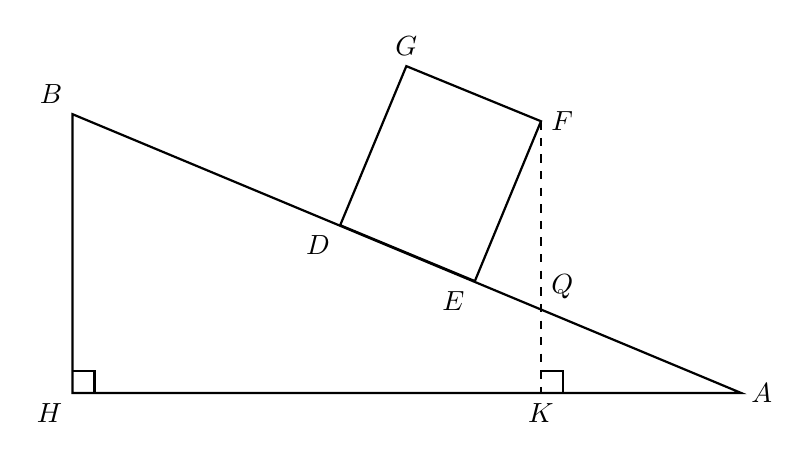
\begin{tikzpicture}[line width=0.8pt]
  % Coordinates (estimated from the figure)
  \coordinate (B) at (0,3.54);
  \coordinate (H) at (0,0);
  \coordinate (A) at (8.49,0);
  \coordinate (K) at (5.95,0);
  \coordinate (Q) at (5.95,1.06);
  \coordinate (F) at (5.95,3.45);
  \coordinate (G) at (4.24,4.15);
  \coordinate (E) at (5.11,1.42);
  \coordinate (D) at (3.40,2.13);

  % Triangle
  \draw (B) -- (H) -- (A) -- cycle;

  % Right angle marks
  \draw (0,0.28) -- (0.28,0.28) -- (0.28,0);
  \draw (5.95,0.28) -- (6.23,0.28) -- (6.23,0);

  % Square DEFG
  \draw (D) -- (E) -- (F) -- (G) -- cycle;

  % Dashed perpendicular FK
  \draw[dashed] (F) -- (K);

  % Labels
  \node[above left] at (B) {$B$};
  \node[below left] at (H) {$H$};
  \node[right] at (A) {$A$};
  \node[below] at (K) {$K$};
  \node[above right] at (Q) {$Q$};
  \node[right] at (F) {$F$};
  \node[above] at (G) {$G$};
  \node[below left] at (E) {$E$};
  \node[below left] at (D) {$D$};
\end{tikzpicture}
\end{document}
